\documentclass[runningheads]{llncs}

% =================================================
% Packages
% =================================================
% Vietnamese characters. The LaTeX default encoding (OT1) has no glyph for
% D-stroke, O-horn, or U-horn, so "Hoa De" and the excluded-letter list in
% Section 3.2 lose those characters silently. T5 (vntex) covers them under
% pdfLaTeX; the fontspec branch covers XeLaTeX and LuaLaTeX.
\usepackage{iftex}
\ifPDFTeX
  \usepackage{lmodern}          % scalable outlines, so T5 does not fall back to bitmaps
  \usepackage[T1,T5]{fontenc}
  \usepackage[utf8]{inputenc}
\else
  \usepackage{fontspec}
  \setmainfont{Latin Modern Roman}
  \setsansfont{Latin Modern Sans}
  \setmonofont{Latin Modern Mono}
\fi

% Evens out the loose interword spacing left by long \texttt{} identifiers.
\usepackage{microtype}

\usepackage{amsmath,amsfonts,amssymb}
\usepackage{graphicx}
\usepackage{booktabs}
\usepackage{tabularx}
\usepackage{array}
\usepackage{xurl}

% Float placement. Without the barrier and the looser fractions, the floats
% queue up and flush out after the bibliography.
%
% The barrier has a cost, though: it turns a float that could not be placed
% into a hole at the foot of the page before the next \section. That is what
% emptied the last quarter of p.11 (Table 5, declared in 6.4, forced out ahead
% of Section 7) and the last fifth of p.3 (Table 1). The tables now carry an
% "h" in their placement specs so they can settle where they are declared
% instead of being deferred into a barrier. If floats still drift too far,
% the next thing to try is dropping the [section] option and placing a manual
% \FloatBarrier only where a figure genuinely must not cross a section.
\usepackage[section]{placeins}
\setcounter{topnumber}{3}
\setcounter{bottomnumber}{2}
\setcounter{totalnumber}{4}
\renewcommand{\topfraction}{0.9}
\renewcommand{\bottomfraction}{0.7}
\renewcommand{\textfraction}{0.07}
% Kept high on purpose: a lower value lets LaTeX open a page for a single
% float and leave the rest blank, which is what produced the near-empty
% figure pages in the first revision.
\renewcommand{\floatpagefraction}{0.85}

% =================================================
% Vertical-space budget
% =================================================
% llncs is generous with vertical glue, and with eight floats, five display
% equations and roughly thirty headings that generosity was costing close to
% two full pages. Everything below tightens glue only; no prose is affected.
% To revert to stock llncs spacing, comment out this whole block.
\makeatletter

% --- Space above/below floats -------------------------------------------
% llncs sets both of these to 8mm (~22.8pt). That is the single largest
% source of the blank bands above and below every figure and table.
\setlength{\textfloatsep}{11\p@ \@plus 2\p@ \@minus 2\p@} % float <-> text, page top/bottom
\setlength{\intextsep}   {9\p@  \@plus 2\p@ \@minus 2\p@} % float placed mid-text
\setlength{\floatsep}    {9\p@  \@plus 2\p@ \@minus 2\p@} % float <-> float
\setlength{\@fptop}{0\p@}          % no leading glue on a float-only page
\setlength{\@fpsep}{8\p@ \@plus 1fil}
\setlength{\@fpbot}{0\p@ \@plus 1fil}

% --- Caption skips -------------------------------------------------------
% Figures caption below the graphic, so \abovecaptionskip is the gap that
% matters there. Tables caption above the body; llncs hardcodes 0pt/10pt
% inside its own table environment, so that environment has to be re-declared.
\setlength{\abovecaptionskip}{5\p@}
\setlength{\belowcaptionskip}{0\p@}
\renewenvironment{table}
   {\setlength\abovecaptionskip{0\p@}%
    \setlength\belowcaptionskip{4\p@}%
    \@float{table}}
   {\end@float}
\renewenvironment{table*}
   {\setlength\abovecaptionskip{0\p@}%
    \setlength\belowcaptionskip{4\p@}%
    \@dblfloat{table}}
   {\end@dblfloat}

% --- Display equations ---------------------------------------------------
% Five numbered displays, each previously carrying ~10pt of glue on both sides.
\setlength{\abovedisplayskip}     {5\p@ \@plus 2\p@ \@minus 2\p@}
\setlength{\belowdisplayskip}     {5\p@ \@plus 2\p@ \@minus 2\p@}
\setlength{\abovedisplayshortskip}{2\p@ \@plus 2\p@}
\setlength{\belowdisplayshortskip}{3\p@ \@plus 2\p@ \@minus 2\p@}

% --- Lists ---------------------------------------------------------------
% Only the contribution list in Section 1 uses this, but llncs opens it with
% 8pt of topsep on each side.
\def\@listI{\leftmargin\leftmargini
            \parsep \z@ \@plus\p@ \@minus\p@
            \topsep 4\p@ \@plus2\p@ \@minus2\p@
            \itemsep \z@}
\let\@listi\@listI
\@listi

% --- Headings ------------------------------------------------------------
% NOTE: this is the one change that visibly departs from the stock LNCS
% layout. llncs asks for 18pt above every heading and 12pt (section) / 8pt
% (subsection) below. Across ~30 headings that is roughly half a page. The
% values below keep the hierarchy legible while reclaiming it. Delete this
% sub-block first if a reviewer objects to the deviation.
\renewcommand\section{\@startsection{section}{1}{\z@}%
                       {-12\p@ \@plus -3\p@ \@minus -3\p@}%
                       {7\p@ \@plus 2\p@ \@minus 2\p@}%
                       {\normalfont\large\bfseries\boldmath
                        \rightskip=\z@ \@plus 8em\pretolerance=10000 }}
\renewcommand\subsection{\@startsection{subsection}{2}{\z@}%
                       {-11\p@ \@plus -3\p@ \@minus -3\p@}%
                       {4\p@ \@plus 2\p@ \@minus 2\p@}%
                       {\normalfont\normalsize\bfseries\boldmath
                        \rightskip=\z@ \@plus 8em\pretolerance=10000 }}
\renewcommand\subsubsection{\@startsection{subsubsection}{3}{\z@}%
                       {-11\p@ \@plus -3\p@ \@minus -3\p@}%
                       {-0.5em \@plus -0.22em \@minus -0.1em}%
                       {\normalfont\normalsize\bfseries\boldmath}}
\renewcommand\paragraph{\@startsection{paragraph}{4}{\z@}%
                       {-9\p@ \@plus -3\p@ \@minus -3\p@}%
                       {-0.5em \@plus -0.22em \@minus -0.1em}%
                       {\normalfont\normalsize\itshape}}

% --- Page filling --------------------------------------------------------
% llncs sets both penalties to 10000, which ends a page one or two lines early
% rather than allow a widow. A high-but-finite penalty still avoids widows
% wherever it is cheap to do so.
\widowpenalty=300
\clubpenalty=300

% llncs calls \LoadClass[twoside]{article}, and article only switches on
% \raggedbottom for ONEside. So this document was running \flushbottom: every
% page is forced to exactly \textheight, and because \parskip is rigid at 0pt
% the entire shortfall gets pumped into the one or two stretchable skips on
% the page -- normally the space around a heading. That is what produced the
% oversized gap around "8.2 Conclusion" on p.14 and the stretched list on p.2.
% \raggedbottom keeps inter-paragraph and heading spacing identical on every
% page and sends the slack to the bottom margin instead.
% (Deviation from stock LNCS, which is flush-bottom. Remove this one line to
% go back.)
\raggedbottom

% --- Line packing --------------------------------------------------------
% The long \texttt{} identifiers (hands126_v1, v2_wrist_centered_mirror) are
% near-unbreakable boxes in a 12.2cm measure. Giving TeX more room to stretch
% lets it settle several paragraphs one line shorter instead of overflowing.
\tolerance=1500
\emergencystretch=2em
\hbadness=1500

\makeatother
% =================================================

\urlstyle{same}

% =================================================
% Page-limit enforcement
% =================================================
% Nothing can guarantee a page count before the document is typeset, but the
% build can be made to refuse to finish quietly once it is. Every compile now
% prints the count, and going over turns into an error rather than something
% discovered on the submission form.
%
%   raise the cap ...... edit \PageLimit
%   downgrade to a note  comment out the \PackageError line
\usepackage{lastpage}
\usepackage{refcount}
\newcommand{\PageLimit}{15}
\AtEndDocument{%
  \typeout{^^J==== PAGE COUNT: \getpagerefnumber{LastPage} of \PageLimit\space ====^^J}%
  \ifnum\getpagerefnumber{LastPage}>\PageLimit\relax
    \PackageError{pagelimit}%
      {Document runs to \getpagerefnumber{LastPage} pages; the limit is \PageLimit}%
      {Cut content, or raise \string\PageLimit\space in main.tex.}%
  \fi
}

\newcolumntype{L}{>{\raggedright\arraybackslash}X}

% =================================================
% Document
% =================================================
\begin{document}

\title{CTU.SignBridge: Protocol- and Artifact-Aware Evaluation of
Low-Resource Vietnamese Sign Recognition}

\titlerunning{Protocol- and Artifact-Aware Sign Recognition}

\author{
Minh-Thai Truong\inst{1}
\and
Huyen-Tran Le Lu\inst{1}
\and
Nhat-Minh Mai\inst{1}
\and
Minh-Nghi Nguyen\inst{1}
\and
Vu-Khoa Vo Tran\inst{1}
\and
Quang-Long Nguyen\inst{1}
\and
Trong-Phuc Chau\inst{1}
}

\authorrunning{M.-T. Truong et al.}

% The student address is one long typewriter string. Without a space after
% each comma LaTeX has almost nowhere legal to break it, so the line runs
% ragged and the closing brace is orphaned onto the next line.
\institute{College of Information and Communication Technology,\\
Can Tho University, Can Tho, Vietnam\\[2pt]
\email{tmthai@ctu.edu.vn}\\
\email{\{tranb2203588, minhb2203567, nghib2203570,
khoab2203560, longb2203562, phucb2203523\}@student.ctu.edu.vn}}

\maketitle

\begin{abstract}
Performer overlap, data partitioning, and incomplete experiment provenance can move low-resource sign-recognition results more than the choice of model does. This paper presents CTU.SignBridge, a protocol- and artifact-aware pipeline for isolated sign recognition from fixed-length hand-landmark sequences collected through a live camera interface, linking canonical performer identities, immutable manifests, versioned splits, processing contracts, and self-describing checkpoints behind fail-closed validity gates. We evaluate five compact neural architectures on a seven-class Hòa Đê workplace-sign profile and a 23-class fingerspelling subset. On Hòa Đê, HandGCN reached the highest mean held-out-performer accuracy, 0.878, and ranked first on all four folds. A matched 120-run experiment then held the test set fixed and varied only what development saw: admitting the target performer into training and validation raised accuracy in all 20 model--performer comparisons, from 0.794 to 0.958 on average. Variation between performers outran the range between architecture means, and the fingerspelling folds supported no stable ranking. Within the profiles we evaluated, performer-aware evaluation and verifiable artifact provenance decide how the resulting numbers should be read.

\keywords{
isolated sign recognition
\and Vietnamese sign recognition
\and hand landmarks
\and held-out-performer evaluation
\and performer exposure
\and artifact provenance
\and reproducibility
}
\end{abstract}

% =================================================
\section{Introduction}
\label{sec:introduction}
Automatic sign recognition can support accessible human--computer interaction, education, and assistive communication. Large-scale isolated-sign benchmarks and pose-based models have advanced the field, but their results transfer poorly to low-resource settings, where a handful of physical performers, incomplete class coverage, and limited independent collection are the norm \cite{li_wlasl_2020,selvaraj_openhands_2022,starner_popsign_2023,desai_asl_citizen_2023}.

In such settings, disjoint sample identifiers prove less than they appear to. When two recordings of the same person land on opposite sides of a split, the model can still lean on that person's morphology, timing, signing style, or capture conditions. Validation deserves particular attention, because validation is what drives early stopping and checkpoint selection: a model tuned against a performer has already met them. We therefore treat an unseen-performer claim as valid only when the target person is absent from training and validation alike.

Artifacts fail in quieter ways. An identity mapping that merges two people, a split regenerated after the fact, a renamed label, a preprocessing step changed between runs, a checkpoint that does not record what produced it --- any one of these can move a number or make it impossible to rebuild. Fixed random seeds do nothing about them. Dataset inventories, split membership, processing contracts, source revisions, and runtime provenance have to be verifiable as well.

This paper presents CTU.SignBridge, a protocol- and artifact-aware pipeline for isolated sign recognition from fixed-length two-hand landmark sequences. We do not propose a new recognition backbone. We examine instead how the evaluation protocol, physical performer identity, and artifact validity shape the interpretation of low-resource results. CTU.SignBridge binds canonical identities, checksummed manifests, versioned splits, processing contracts, and self-describing checkpoints behind fail-closed validity gates.

We evaluate two profiles: a seven-class Hòa Đê community-origin workplace-sign profile with 445 usable samples from four complete-coverage performers, and a 23-class fingerspelling subset with 793 usable samples from five physical performers, only two of whom cover every class. Five compact architectures share one optimization budget: HandGCN, TCN, CNN, bidirectional LSTM, and BiGRU with attention. Our principal protocol holds one performer out of both training and validation. A matched control then sets performer-unseen against performer-exposed development on the same fixed, disjoint test samples.

That matched experiment comprises 120 research-valid runs. Exposing the target performer during training and validation raised fixed-test accuracy in all 20 model--performer comparisons, from 0.794 to 0.958 on average. On Hòa Đê, HandGCN reached the highest mean held-out-performer accuracy, 0.878, and ranked first on all four folds; the two complete fingerspelling folds supported no stable ranking.

We contribute:
\begin{enumerate}
    \item a fail-closed pipeline that links canonical physical-performer identities to immutable manifests, versioned splits, processing contracts, and self-describing checkpoints;
    \item a matched 120-run experiment that measures what target-performer exposure during training and validation is worth on fixed disjoint test sets;
    \item held-out-performer comparisons of five compact architectures across two low-resource recognition profiles;
    \item reliability evidence drawn from identity reconciliation, augmentation semantics, checkpoint provenance, and deterministic execution.
\end{enumerate}


\section{Related Work}
\label{sec:related_work}
\subsection{Landmark-Based Isolated Sign Recognition}

Large-scale datasets such as WLASL, PopSign ASL, and ASL Citizen have expanded isolated-sign recognition across web-video, smartphone, and community-sourced settings \cite{li_wlasl_2020,starner_popsign_2023,desai_asl_citizen_2023}. Their scale and performer diversity contrast with low-resource collections, where identity and split decisions can strongly affect reported results.

Pose- and landmark-based methods reduce appearance dependence by modeling structured keypoint sequences. OpenHands supports pose-based transfer across languages, while skeleton-aware, hand-model-aware, multimodal, and part-wise approaches model spatial and temporal relations more explicitly \cite{selvaraj_openhands_2022,jiang_samslr_2021,hu_signbert_2021,gruber_modalities_2021,lee_p3d_2023}. We adopt a fixed two-hand landmark representation and make no claim to improve on it. Our attention goes to protocol and artifact validity instead.

\subsection{Low-Resource and Signer-Independent Evaluation}

Signer-independent evaluation is especially difficult in low-resource settings \cite{sincan_chalearn_2021,holmes_low_resource_2022}. Separating samples is not enough when several identifiers turn out to be one physical person, or when a single collection account aggregates several performers. We therefore take canonical physical-performer identity as the unit of independence and keep the target performer out of both training and validation.

Vietnamese sign-recognition studies have explored dynamic-object extraction, MediaPipe-based alphabet recognition, and cross-attention video models \cite{pham_vsl_dynamic_2021,tran_vsl_alphabet_2025,chu_crossvivit_2025}. Neither their tasks nor their participant populations are directly comparable to ours. We are correspondingly careful with names: Hòa Đê is a community-origin workplace-sign profile, not a standardized vocabulary or a validated regional dialect, and our second profile is a 23-class fingerspelling subset, not a complete alphabet.

\subsection{Artifact Documentation and Reproducibility}

Datasheets and Model Cards promote structured reporting of datasets, models, evaluation conditions, and limitations \cite{gebru_datasheets_2021,mitchell_model_cards_2019}. OpenML-Python and Git-Theta offer complementary mechanisms for experiment sharing and model version control \cite{feurer_openml_python_2021,kandpal_git_theta_2023}. We apply those principles as machine-checkable links running from identity mappings and manifest checksums through splits, contracts, and source revisions to the checkpoint itself. Where the chain breaks, the run is excluded rather than kept with a warning attached.

\section{Data and Representation}
\label{sec:data}
% Plain math italic, not \mathbf: the symbol is introduced once and never
% reused, so a bold X only reads as an accidental bold word mid-sentence.
Each sample is represented by
$X\in\mathbb{R}^{60\times126}$, where each frame contains
$2\times21\times3=126$ coordinates from two MediaPipe hand slots.
The $x$ and $y$ values are image-normalized, while $z$ is a relative
depth estimate rather than a metric three-dimensional position.
Missing-hand slots are zero-valued. All experiments use the
\texttt{hands126\_v1} processing contract. Table~\ref{tab:profiles}
summarizes the two profiles we evaluate.

\begin{table}[htbp]
\centering
\caption{Evaluated recognition profiles. Performer counts are given as
canonical physical performers over those with complete class coverage.}
\label{tab:profiles}
\small
\setlength{\tabcolsep}{4pt}
\renewcommand{\arraystretch}{1.08}

\begin{tabularx}{\linewidth}{
    >{\raggedright\arraybackslash}p{3.7cm}
    c
    c
    c
    >{\raggedright\arraybackslash}X
}
\toprule
\textbf{Profile}
& \textbf{Classes}
& \textbf{Samples}
& \textbf{Perf.}
& \textbf{Evaluation} \\
\midrule
Hòa Đê workplace signs
& 7 & 445 & 4/4
& Four performer-held-out folds \\
Fingerspelling subset
& 23 & 793 & 5/2
& Two complete-coverage folds \\
\bottomrule
\end{tabularx}
\end{table}

\subsection{Hòa Đê Workplace-Sign Profile}
\label{subsec:hoa_de_profile}

The Hòa Đê profile contains seven workplace signs:
\texttt{rang-muoi}, \texttt{tom}, \texttt{lot-da-ca},
\texttt{lot-vo-tom}, \texttt{cat-ky}, \texttt{danh-vay-ca}, and
\texttt{cat-dau-ca}.

Four adult performers, denoted H01--H04, contributed 445 usable samples,
and all four covered all seven classes. H03 is the originating Deaf
performer. H01, H02, and H04 were instructed performers who had not
habitually used the vocabulary before collection.

Source glosses were entered during capture, with help from a family
member of H03 who communicated with them regularly. We therefore treat
the labels as source annotations grounded in H03's own communication
practice. They are not independent linguistic validation, and we do not
present them as such.

\subsection{Fingerspelling Profile}
\label{subsec:fingerspelling_profile}

The fingerspelling subset contains 793 usable samples across 23 classes:

\begin{equation}
\begin{aligned}
\mathcal{C}_{\mathrm{FS}}=\{&
\mathrm{A},\mathrm{B},\mathrm{C},\mathrm{D},\mathrm{E},
\mathrm{G},\mathrm{H},\mathrm{I},\mathrm{K},\mathrm{L},
\mathrm{M},\mathrm{N},\\
&
\mathrm{O},\mathrm{P},\mathrm{Q},\mathrm{R},\mathrm{S},
\mathrm{T},\mathrm{U},\mathrm{V},\mathrm{X},\mathrm{Y},
\mathrm{Z}\}.
\end{aligned}
\label{eq:fingerspelling_classes}
\end{equation}

This profile is not a complete Vietnamese fingerspelling inventory. It
excludes the Latin letters F, J, and W, as well as the
Vietnamese-specific letters Ă, Â, Đ, Ê, Ô, Ơ, and Ư.

Five physical performers contributed samples, but only F01 and F02
covered all 23 classes. Together, they contributed approximately 89\%
of the usable samples. F01 and F02 correspond to H01 and H02,
respectively; profile-specific pseudonyms are retained to keep the two
collection inventories and split artifacts unambiguous.

One of those performers turned out to have been recorded under two
collection identifiers, \texttt{S005} and \texttt{S007}. We reconciled
the pair to a single physical person in the canonical identity mapping.
Left alone, it would have inflated the profile to six performers where
there are five, and nothing would have stopped a split from placing one
person on both sides of itself.

\subsection{Session and Motion Audits}
\label{subsec:session_motion_audits}

Spreadsheet handling converted several early Hòa Đê session identifiers
into scientific-notation strings, and distinct source identifiers lost
the digits that told them apart. Sample identifiers survived intact, so
no sample is ambiguous, but exact historical session counts cannot be
reconstructed for every record. We therefore describe the collection as
multi-session and make no claim of session-disjoint evaluation.

A descriptive motion audit computed the mean frame-to-frame $\ell_1$
landmark displacement per class. Z, which is dynamic by design, scored
approximately 0.357. Q scored approximately 0.375, higher than Z despite
being intended as a static handshape, and roughly 97\% of its samples
exceeded 0.2. Manual inspection confirmed the cause: the
recordings are contaminated with movement that does not belong to the
sign.

We kept Q in the frozen manifest rather than dropping it, so that the
evaluated task definition stays intact and comparable, and we flag every
fingerspelling result with this caveat. The class is marked for
recollection in a future dataset version.

Raw videos were not retained. Participant-level landmark sequences
remain private, so the conclusions concern the frozen
\texttt{hands126\_v1} representation.

\section{Protocol- and Artifact-Aware Pipeline}
\label{sec:pipeline}
CTU.SignBridge treats research validity as a machine-checkable property of the artifacts. A completed training process is eligible for reporting only when its identity, dataset, split, processing, source, runtime, and checkpoint provenance can be verified. Fig.~\ref{fig:pipeline} traces those artifacts and the two gates each run has to clear.

\begin{figure}[tbp]
\centering
% Portrait diagram: at 0.56\linewidth it stood 9.8cm tall, half the text
% block. 0.52 keeps the node labels legible and returns ~0.7cm.
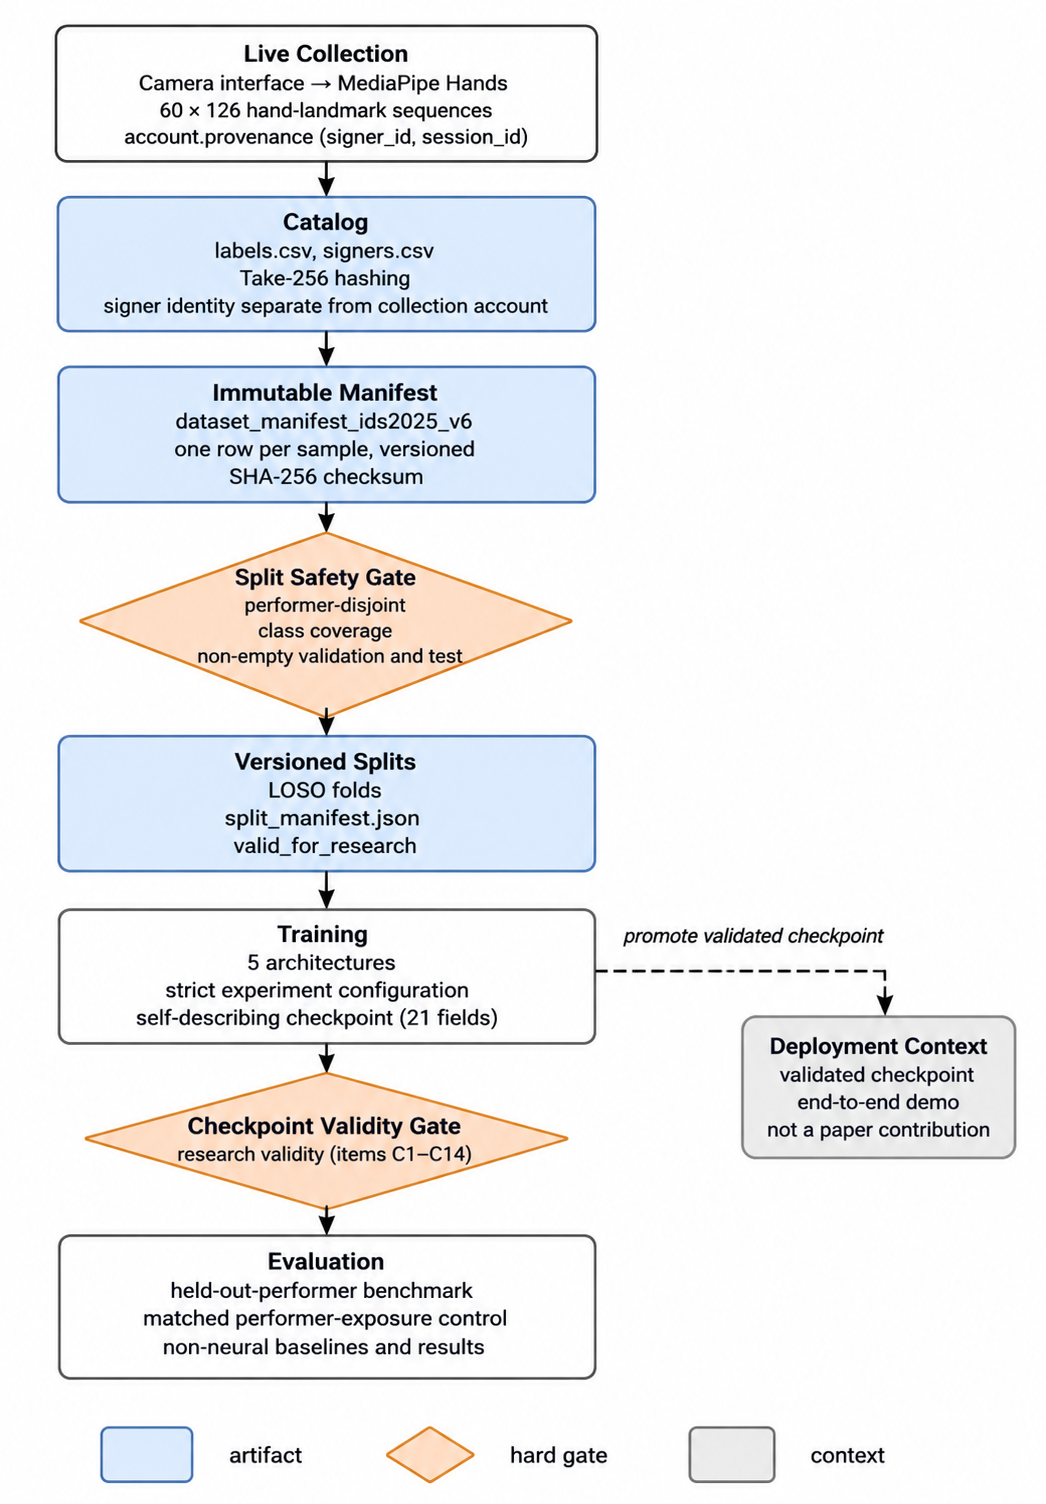
\includegraphics[
    width=0.52\linewidth,
    trim=8mm 5mm 8mm 5mm,
    clip
]{Figures/Figure1_pipeline.png}
\caption{Artifact-versioned CTU.SignBridge pipeline. Research results
are produced only after the split and checkpoint validity gates pass;
the deployment branch is shown only as system context.}
\label{fig:pipeline}
\end{figure}

\subsection{Identity, Manifest, and Split Artifacts}

Three things that are easy to conflate are kept apart in the identity catalog: the collection account, the canonical physical performer (\texttt{signer\_id}), and the recording session (\texttt{session\_id}). Separating them handles the problem in both directions, one account standing for several people and one person appearing under several historical identifiers. Every performer-disjoint check runs against the canonical physical-person mapping.

Class names need the same care. The vocabulary catalog defines profile-specific class identifiers, display labels, and storage slugs, and the slugs are Telex-style and vocabulary-aware so that two classes do not collide once Vietnamese diacritics are stripped.

Each processed sample is then indexed by an immutable manifest recording its profile, class, performer, available session provenance, storage reference, and processing contracts. A SHA-256 checksum binds that manifest to versioned train--validation--test splits and to every checkpoint downstream of them. When we correct an inventory we version it; we do not overwrite the previous one.

The split gate is where all of this becomes enforceable. It rejects unresolved identities, physical-performer overlap, missing class coverage, empty validation or test partitions, and labels outside the active profile. The fold counts show the gate doing its work: Hòa Đê admits four complete held-out-performer folds, while fingerspelling admits only F01 and F02 as complete 23-class test folds.

\subsection{Processing and Augmentation Contracts}

Training is bound to explicit preprocessing and augmentation versions; the experiments reported here use \texttt{v2\_wrist\_centered\_mirror}. An earlier version mirrored horizontally in image coordinates, after the sequence had already been wrist-centered:
\begin{align}
\text{v1, incorrect:}\quad x' &= 1-x, \label{eq:mirror_v1}\\
\text{v2, corrected:}\quad x' &= -x. \label{eq:mirror_v2}
\end{align}
Applied uniformly, Eq.~\eqref{eq:mirror_v1} does preserve pairwise distances, which is why it survived casual inspection. It nonetheless breaks the contract twice over: it shifts the origin away from the wrist, and it maps zero-valued missing-hand slots onto nonzero coordinates, so an absent hand becomes a hand at $x'=1$.

Reflecting about the wrist instead, as in Eq.~\eqref{eq:mirror_v2}, fixes both. We follow it by exchanging the left- and right-hand slots; missing slots stay at zero. The corrected contract passed 22 checks with no failures, covering wrist-origin, distance, span, empty-slot, padding, mask, involution, valid-frame, and coordinate-range properties. Temporal masking is disabled, since zero already means both ``missing hand'' and ``padding''.

\subsection{Self-Describing Checkpoints and Validity Gates}

A research checkpoint carries 21 required fields. They describe the model structure and input dimensions, the profile-specific label map, the dataset and split versions, the manifest checksum, the processing contracts, the seed and training configuration, the source revision and runtime environment, and finally how the checkpoint was selected and what it scored.

Every run is marked \texttt{smoke\_test} or \texttt{research}, and the default is \texttt{smoke\_test}, so a run has to earn the research label rather than inherit it. An early batch of 60 completed executions lacked sufficient provenance under this rule. We rejected all 60 and repeated them under the research protocol rather than patching metadata in after the fact, which would have defeated the purpose of recording it.

The post-training gate then checks 14 criteria: run purpose, required fields, artifact compatibility, manifest agreement, split validity, profile-label consistency, environment provenance, checkpoint restoration, nonempty test data, and successful completion. A run that cannot establish its validity is excluded.

\subsection{Deterministic Execution and Aggregation}

Strict execution fixes the Python, NumPy, and PyTorch seeds, deterministic PyTorch and cuDNN behavior, CUDA workspace settings, split artifacts, dataset ordering, and \texttt{num\_workers=0}. Only checkpoints that clear both the split gate and the research-validity gate reach aggregation. The public artifact package will carry code, weights, schemas, checksums, metrics, audit scripts, and environment metadata. Participant-level sequences stay private.

\section{Experimental Design}
\label{sec:experimental_design}
All models used Adam with learning rate $10^{-3}$, weight decay $10^{-4}$, batch size 32, dropout 0.3, cosine annealing over at most 80 epochs, gradient clipping at 1.0, and early stopping with patience 10 on validation macro-F1. Experiments used seeds 42, 43, and 44, deterministic execution, and \texttt{num\_workers=0}. The environment was WSL2 Linux with Python 3.11.15, PyTorch 2.0.0+cu117, NumPy 1.26.2, cuDNN 8.5.0, and an RTX 3050 Laptop GPU.

\subsection{Held-Out-Performer Evaluation}

For each eligible target performer, every sample from that performer forms the test fold, and training and validation draw only on the others:
\begin{equation}
\mathcal{P}_{\mathrm{train}}\cap\mathcal{P}_{\mathrm{test}}
=
\mathcal{P}_{\mathrm{val}}\cap\mathcal{P}_{\mathrm{test}}
=
\varnothing.
\label{eq:performer_disjoint}
\end{equation}
Note that Eq.~\eqref{eq:performer_disjoint} constrains performer sets, not sample sets; this is the distinction the rest of the paper turns on. Hòa Đê yields $5\times4\times3=60$ runs and fingerspelling $5\times2\times3=30$. We average performer-level results over the three seeds, then average across eligible performers to obtain an architecture mean. Performers are the independent evaluation units, not samples and not seeds.

\subsection{Matched Performer-Exposure Experiment}

To isolate what performer exposure alone is worth, we hold the test set still and vary only what development sees (Fig.~\ref{fig:matched_protocol}). For each Hòa Đê performer, roughly half the samples form a fixed, class-balanced test set; the remainder become an exposure pool. Protocol A keeps the target performer out of training and validation. Protocol B moves disjoint exposure-pool samples into both development partitions, leaving the fixed test sample identifiers untouched:
\begin{equation}
\mathcal{T}_p\cap
\left(
\mathcal{D}^{B}_{\mathrm{train}}\cup
\mathcal{D}^{B}_{\mathrm{val}}
\right)=\varnothing.
\label{eq:test_disjoint}
\end{equation}
Matching matters here, so the added target-performer training samples displace class-matched samples from other performers. Training size and per-class training counts therefore stay fixed across the two protocols. Only validation composition changes, and it changes deliberately, because checkpoint selection is half of what we are measuring.

For model $m$ and performer $p$, the exposure gap is the difference between the two accuracies on that same fixed test set:
\begin{equation}
\Delta_{m,p}=a^B_{m,p}-a^A_{m,p}.
\label{eq:exposure_gap}
\end{equation}
The experiment comprises $5\times4\times2\times3=120$ valid runs. One caveat travels with Eq.~\eqref{eq:exposure_gap}: because early session provenance is incomplete, $\Delta_{m,p}$ may absorb session-related similarity alongside performer-related similarity.

\begin{figure}[tbp]
\centering
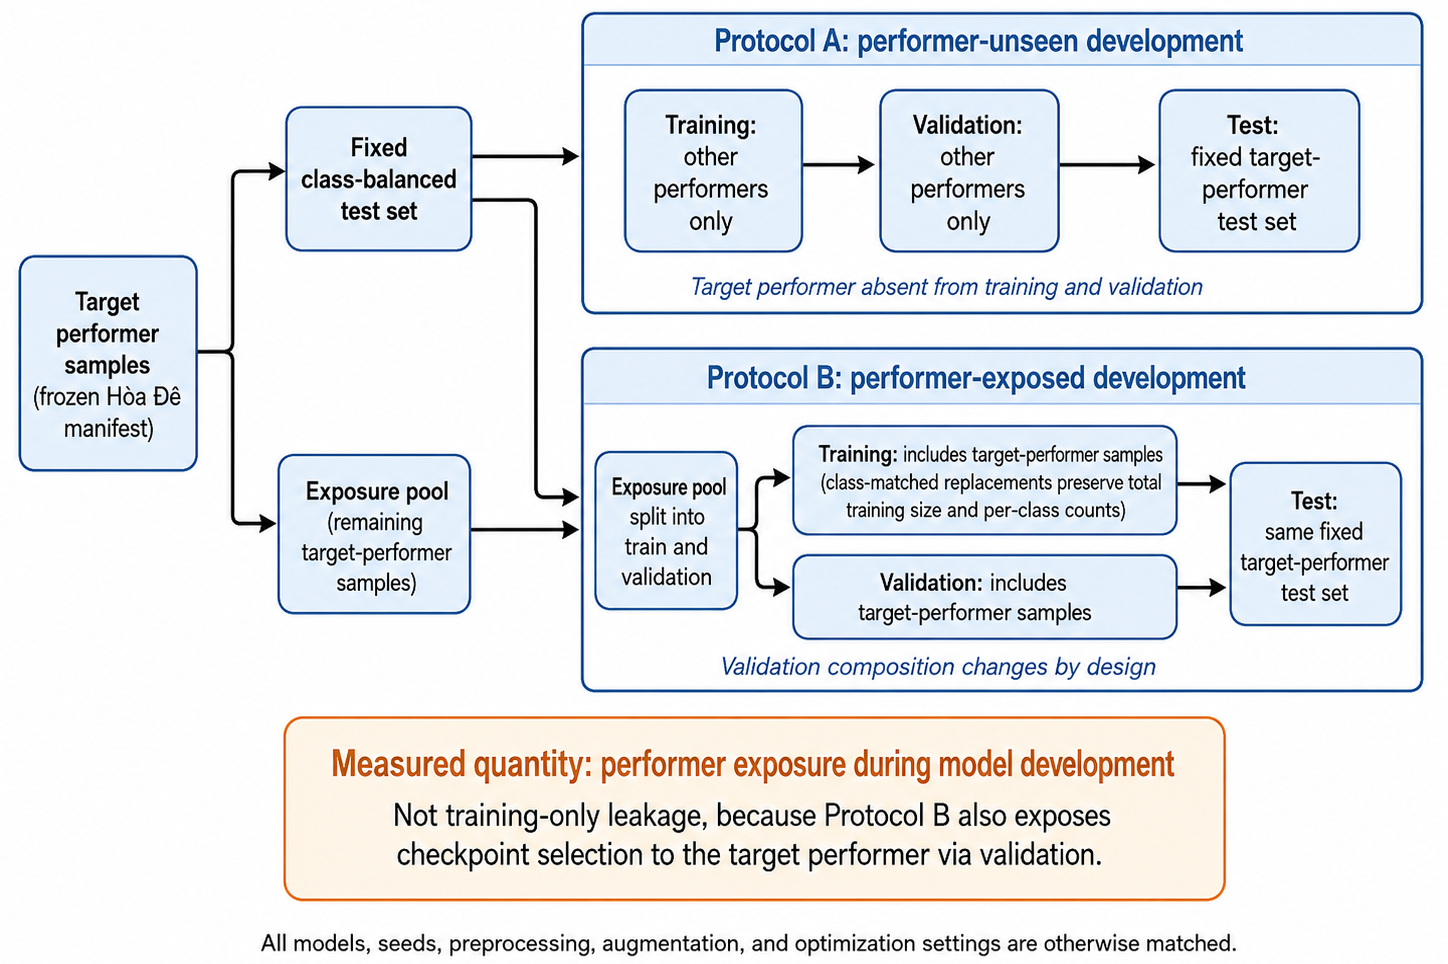
\includegraphics[width=0.90\linewidth]{Figures/Figure2_matched_protocol.png}
\caption{Matched performer-exposure protocol. Both conditions use the same fixed target-performer test set; Protocol A excludes the target performer from training and validation, while Protocol B introduces disjoint target-performer samples into both development partitions.}
\label{fig:matched_protocol}
\end{figure}

\subsection{Models, Baselines, and Metrics}

\begin{table}[htbp]
\centering
\caption{Evaluated neural architectures.}
\label{tab:models}
\small
\setlength{\tabcolsep}{4pt}
\renewcommand{\arraystretch}{1.1}
\begin{tabularx}{\linewidth}{l L r}
\toprule
\textbf{Model} & \textbf{Core configuration} & \textbf{Parameters} \\
\midrule
HandGCN & 42-node hand graph; two distance-aware GCN layers; part pooling; temporal attention & 135,711 \\
TCN & Three dilated temporal blocks; 64 channels; temporal attention & 133,960 \\
CNN & Three temporal convolutions; max pooling; global average pooling & 281,162 \\
LSTM & Two bidirectional layers; hidden size 64; global average pooling & 206,343 \\
BiGRU+Attn & Two bidirectional GRU layers; hidden size 64; self-attention & 206,471 \\
\bottomrule
\end{tabularx}
\end{table}

Table~\ref{tab:models} lists the five architectures and their parameter counts. Alongside them we evaluated uniform-chance, majority-class, Euclidean nearest-centroid, and Euclidean 1-NN baselines on flattened $60\times126$ sequences, keeping the zero-valued missing-hand slots so that the baselines see exactly what the networks see. Accuracy and macro-F1 were recorded for every run, and validation macro-F1 selected the checkpoint. With four performers as our independent units, we keep the analysis descriptive and report no sample-level significance tests.

\subsection{Reproducibility Protocols}

Our same-code test repeated two executions of commit \texttt{28f0393} for HandGCN, CNN, and TCN, holding the RTX 3050 environment, seed, split, and 80-epoch configuration constant, and compared model-state tensors, predictions, metrics, and metadata exactly. A second test compared 90 corresponding configurations across commits \texttt{0475b78} and \texttt{7ee3fbd}. Since the source revisions differ there, we read that result as optimization robustness and not as determinism.

\section{Results}
\label{sec:results}
All reported runs passed the split and research-validity gates.

\subsection{Target-Performer Exposure}

Target-performer exposure increased fixed-test accuracy in all 20 architecture--performer comparisons. The mean increase was 0.164, the median was 0.154, and the range was 0.024--0.304. Averaged across models and seeds, H01--H04 improved from 0.836, 0.739, 0.905, and 0.694 under Protocol A to 0.953, 0.956, 0.973, and 0.949 under Protocol B. Overall mean accuracy increased from 0.794 to 0.958. Fig.~\ref{fig:exposure_gap} shows the same result performer by performer.

\begin{figure}[tbp]
\centering
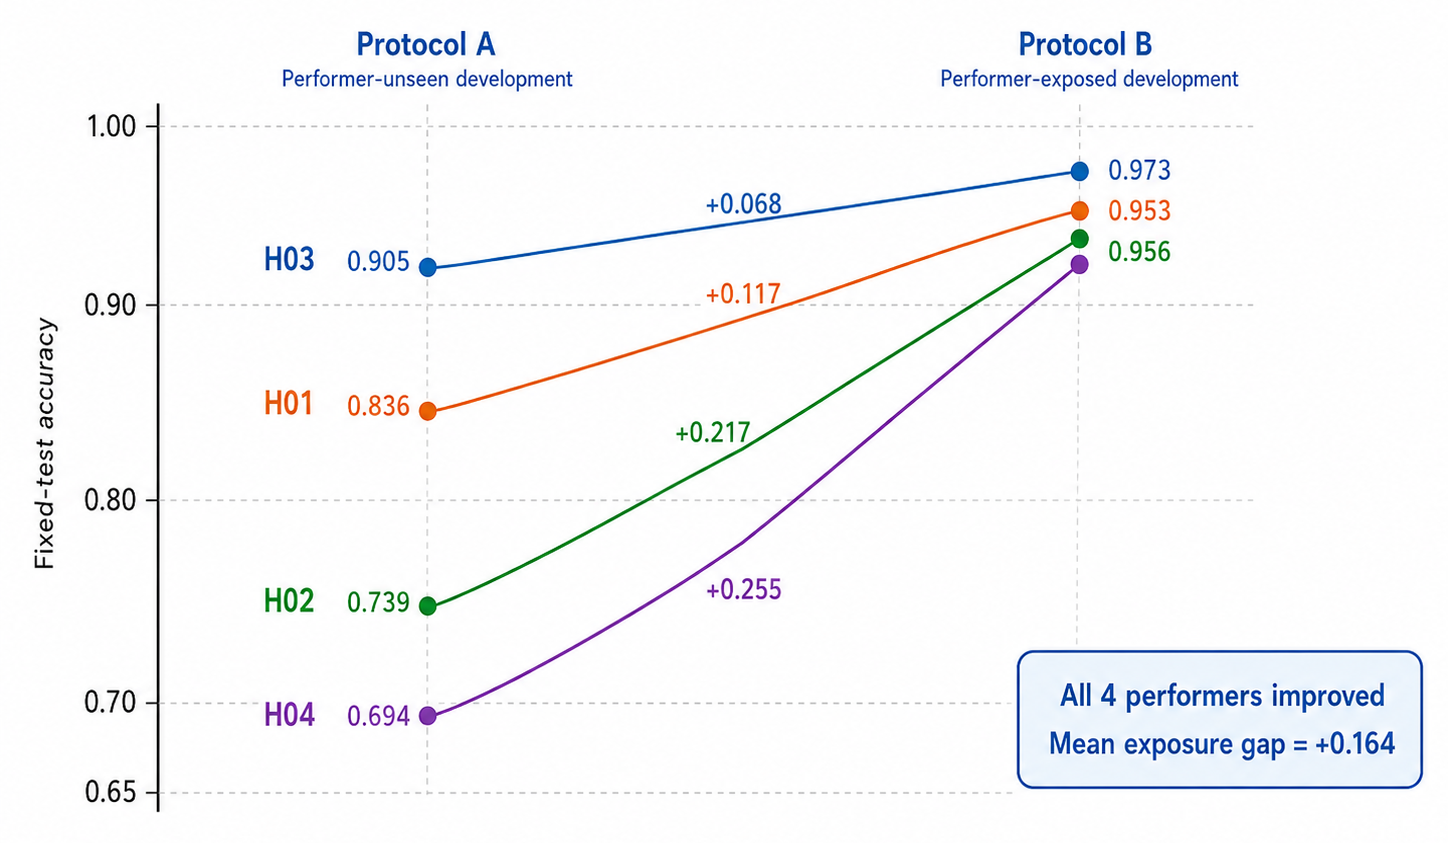
\includegraphics[width=0.84\linewidth]{Figures/Figure3_exposure_gap.png}
\caption{Fixed-test accuracy under performer-unseen and performer-exposed development, averaged over five architectures and three seeds. All four target performers improved; the mean exposure gap was 0.164.}
\label{fig:exposure_gap}
\end{figure}

This gap exceeded the 0.116 range among Hòa Đê architecture means, though the two are not statistically equivalent effect measures and we do not treat them as such. Our claim is descriptive: within this dataset and this configuration set, the protocol difference was larger than the spread among model-family means. One point of interpretation matters. Protocol B exposes the target performer to optimization and to validation-based selection at once, so what we measured is performer exposure across model development as a whole, not training-only leakage.

\subsection{Hòa Đê Held-Out-Performer Results}

The Hòa Đê reference accuracies were 0.143 for uniform chance, 0.146 for the majority class, 0.552 for nearest centroid, and 0.719 for 1-NN.

\begin{table}[htbp]
\centering
\caption{Hòa Đê held-out-performer accuracy. Cells are means over three seeds; SD is computed across the four performer means.}
\label{tab:hoa_de}
\small
\setlength{\tabcolsep}{3.8pt}
\renewcommand{\arraystretch}{1.08}
\begin{tabularx}{\linewidth}{L c c c c c c}
\toprule
\textbf{Model} & \textbf{H01} & \textbf{H02} & \textbf{H03} & \textbf{H04} & \textbf{Mean} & \textbf{SD} \\
\midrule
HandGCN & 0.941 & 0.823 & 0.971 & 0.775 & 0.878 & 0.094 \\
CNN & 0.829 & 0.748 & 0.946 & 0.657 & 0.795 & 0.123 \\
TCN & 0.846 & 0.701 & 0.898 & 0.641 & 0.772 & 0.120 \\
LSTM & 0.804 & 0.736 & 0.924 & 0.600 & 0.766 & 0.135 \\
BiGRU+Attn & 0.776 & 0.771 & 0.838 & 0.663 & 0.762 & 0.073 \\
\bottomrule
\end{tabularx}
\end{table}

\begin{figure}[tbp]
\centering
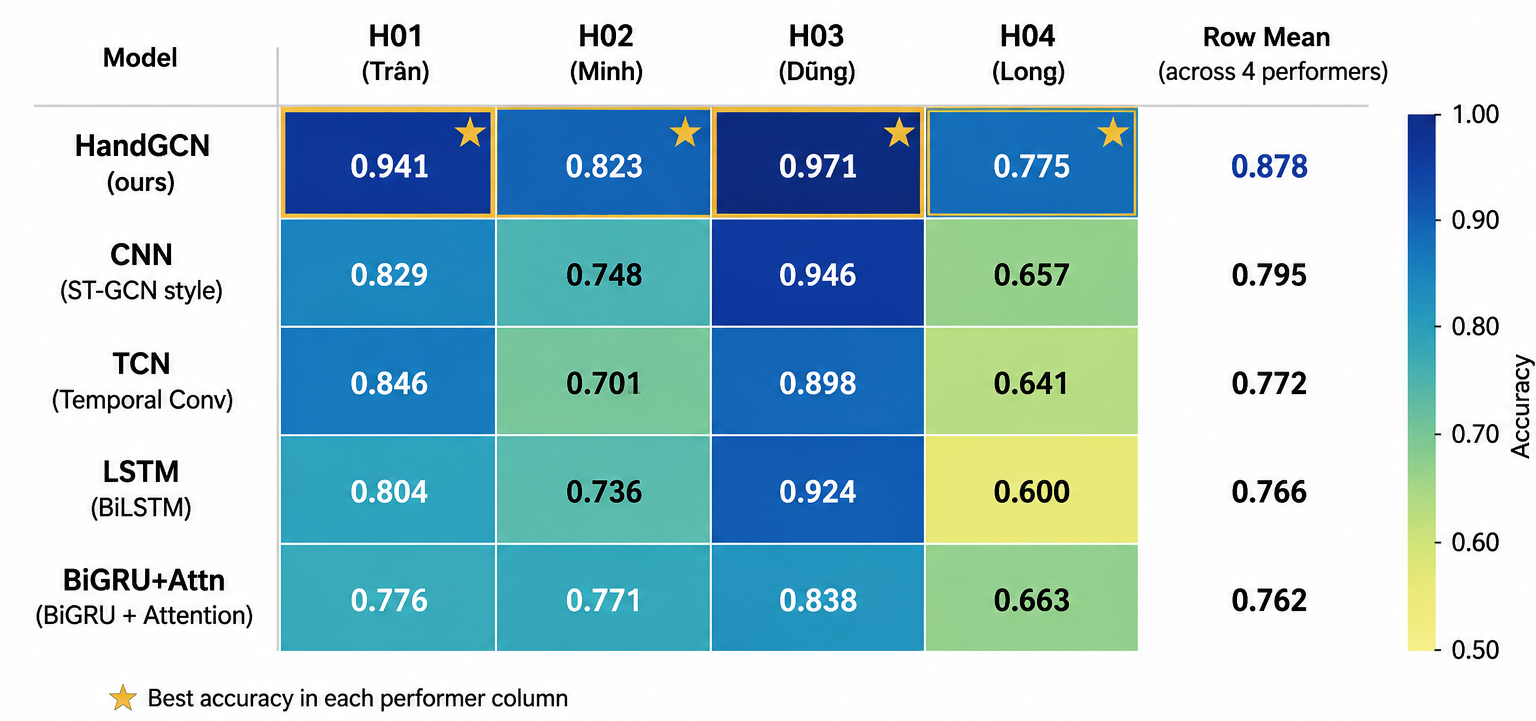
\includegraphics[width=0.95\linewidth]{Figures/Figure4_hoa_de_heatmap.png}
\caption{Held-out-performer accuracy on the Hòa Đê profile, per architecture
and per target performer, with row means across the four performers. Stars
mark the best architecture in each performer column. The same values appear
in Table~\ref{tab:hoa_de}.}
\label{fig:hoa_de_heatmap}
\end{figure}

Table~\ref{tab:hoa_de} reports the full fold-by-fold results, and
Fig.~\ref{fig:hoa_de_heatmap} shows the same matrix as a heatmap, where the
column-wise structure is easier to read off. HandGCN ranked first on all four folds and took the highest mean accuracy, 0.878, with CNN second at 0.795 and a spread of 0.116 across architecture means. The margins behind that sweep are uneven: 0.095, 0.052, 0.025, and 0.112 over the runner-up at H01 through H04. The narrowest of them, 0.025 over CNN at H03, is thin enough that we present the sweep as a description of these three seeds rather than as a stable property of the architecture. Averaged across models, H01--H04 scored 0.839, 0.756, 0.916, and 0.667, a spread of 0.249. Performer-level variation was thus descriptively larger than architecture-level variation. H03 proved easiest and H04 hardest; H03 is also the originating Deaf performer, but with exactly one originator in the profile we cannot separate that role from anything else about them, and we draw no originator effect from it.

\subsection{Fingerspelling Results}

\begin{table}[htbp]
\centering
\caption{Accuracy on the 23-class fingerspelling subset, averaged over three seeds.}
\label{tab:fingerspelling}
\small
\setlength{\tabcolsep}{7pt}
\renewcommand{\arraystretch}{1.08}
\begin{tabular}{lccc}
\toprule
\textbf{Model} & \textbf{F01} & \textbf{F02} & \textbf{Mean} \\
\midrule
BiGRU+Attn & 0.885 & 0.752 & 0.819 \\
HandGCN & 0.829 & 0.774 & 0.802 \\
TCN & 0.866 & 0.703 & 0.785 \\
LSTM & 0.854 & 0.695 & 0.775 \\
CNN & 0.840 & 0.697 & 0.769 \\
\bottomrule
\end{tabular}
\end{table}

In Table~\ref{tab:fingerspelling}, BiGRU+Attn took the highest two-fold mean and HandGCN came second, but the two folds disagree about which is better: BiGRU+Attn wins F01 and HandGCN wins F02. The architecture means span only 0.050, and several models differ more than that between the two performers alone. Two folds that contradict each other, separated by less than the within-model performer gap, do not support a stable fingerspelling ranking, and we do not report one.

\subsection{Reproducibility Evidence}

Repeating commit \texttt{28f0393} for HandGCN, CNN, and TCN under one fixed environment, seed, and split reproduced bit-identical model states, predictions, and metrics, across 24 checks per model. The cross-revision comparison came out weaker: over 90 paired configurations predictions were unchanged and metrics agreed to four decimals, but some HandGCN parameters differed by roughly $10^{-6}$.

We therefore establish same-code determinism only for that commit, those three architectures, and that one RTX 3050 environment, and we claim nothing past it. The cross-revision result we read as behavioral stability, not as byte-identical models.

\section{Discussion and Reliability Evidence}
\label{sec:discussion}
\subsection{Protocol and Performer Effects}

The matched experiment is our central result, and its lesson is narrow but firm: disjoint test samples did not, on their own, establish unseen-performer generalization once other samples from the same person were available during development. Protocol A asks what a model does with a person it has never met. Protocol B asks what it does with new samples from a person who shaped both its weights and its checkpoint. Both are legitimate questions. They are not the same question, and a paper that reports one while claiming the other has overstated its result.

Three numbers sit side by side here. The mean exposure gap was 0.164; the spread across architecture means was 0.116; the spread across performers was 0.249. We are not claiming these are commensurable effect measures, and none of this proves that protocol dominates architecture in general. What it does show is that in this low-resource setting, who was recorded and how the partitions were drawn moved the conclusions at least as much as which network we trained. The practical reading is that recruiting one more independent performer is likely worth more than collecting many more repetitions from the people we already have.

\subsection{Architecture Interpretation}

HandGCN's explicit hand-topology bias plausibly helps it model the coordinated spatial and temporal structure of the Hòa Đê signs, which are predominantly dynamic. We offer that as a reading, not a finding: we ran no component ablations, and the two fingerspelling folds disagreed with each other about the best architecture. What the evidence supports is bounded to the configuration we evaluated. HandGCN was strongest on Hòa Đê. That is not the same as being the right architecture for Vietnamese sign recognition.

\subsection{Reliability Evidence}

\begin{table}[htbp]
\centering
\caption{Representative validity risks and safeguards.}
\label{tab:reliability}
\small
\setlength{\tabcolsep}{3pt}
\renewcommand{\arraystretch}{1.08}

\begin{tabularx}{\linewidth}{
    >{\raggedright\arraybackslash}p{2.2cm}
    >{\raggedright\arraybackslash}X
    >{\raggedright\arraybackslash}X
}
\toprule
\textbf{Risk}
& \textbf{Potential consequence}
& \textbf{Control} \\
\midrule
Identity ambiguity
& Hidden overlap or inflated performer count
& Canonical physical-person mapping \\

Performer exposure
& Misstated unseen-person generalization
& Performer-held-out gate and explicit protocol labels \\

Mirror semantics
& Invalid wrist origin and missing-hand encoding
& Versioned correction and 22 checks \\

Incomplete provenance
& Invalid runs entering aggregation
& Fail-closed gate; affected runs repeated \\

Q contamination
& Spurious temporal cue
& Caveated reporting and planned recollection \\

Session and storage
& Uncertain session separation or restoration
& String identifiers, checksums, and link audits \\
\bottomrule
\end{tabularx}
\end{table}

Table~\ref{tab:reliability} pairs each validity risk we encountered with the control that answers it. Two of them deserve expanding on. A storage audit found 538 incorrect backup links among 937 inspected records. The local processed files used for training were correct, so no reported metric changed, but a restoration attempted through those links would have failed. We report the audit precisely because of that gap: computational repeatability and long-term artifact recoverability are different properties, and passing the first says nothing about the second.

Determinism has the same blind spot. A run can be bit-identical on every rerun and still be scientifically worthless if its identity mapping, split, label namespace, augmentation semantics, or manifest is wrong; it will simply reproduce the wrong answer reliably. We therefore treat reproducibility as layered evidence rather than a single property: stable execution, compatible versioned artifacts, valid performer semantics, recoverable provenance, and data-quality limitations stated out loud.

\subsection{Implications}

Three recommendations follow for low-resource sign recognition. State which generalization you are claiming: new samples from known performers, new sessions, unseen performers, or new devices and sites. These are four different claims, and only one of them is usually tested. Compare architectures on the same frozen manifest, splits, preprocessing, augmentation, seeds, metrics, and checkpoint rule, so that the comparison is about the architectures. And treat identity overlap, checksum mismatch, label inconsistency, outdated contracts, and incomplete provenance as grounds for excluding a run, not as warnings to be read past. A warning that nobody acts on is indistinguishable from no warning at all.

\section{Limitations and Conclusion}
\label{sec:conclusion}
\subsection{Limitations}

Our study covers two small, closed-set profiles. Hòa Đê holds seven workplace signs and four complete-coverage performers; fingerspelling holds 23 classes and five physical performers, of whom only F01 and F02 cover all classes, between them contributing approximately 89\% of the usable samples. Three seeds reduce optimization variability, but seeds are not participants, and no number of them adds participant-level replication. Our analysis is descriptive for that reason.

One consequence deserves stating on its own. We report cell means over three seeds but not the dispersion within a cell, so the 0.116 spread across architecture means arrives without an error bar and we cannot say how much of it is optimization noise. The architecture ranking should be read as provisional to exactly that extent, and the 0.025 margin at H03 is the clearest place where it might not hold. The exposure result is less exposed to the same doubt, since it is roughly $1.4\times$ larger and holds in all 20 cells with a minimum of 0.024, but we would rather name the weakness than let its size stand in for an argument.

Participant roles are heterogeneous. H03 originated the Hòa Đê vocabulary while H01, H02, and H04 were instructed performers, and we cannot separate that role from fluency, morphology, timing, or capture conditions. Q carries known motion contamination and should be recollected.

The matched experiment cannot guarantee session-disjointness, since some early session identifiers lost precision before we could preserve them. Protocol B also bundles two things together: target-performer influence on optimization, and target-performer influence on validation-based checkpoint selection. Its 0.164 gap is therefore a within-dataset exposure estimate. It is neither a universal causal effect nor a training-only one.

Our models see only frozen hand-landmark sequences. Raw videos were not retained, so body, face, texture, and context are simply unavailable to them. All five architectures also share a single optimization budget. That buys procedural comparability, but it means no architecture here was tuned to its own best, and parameter counts still vary by roughly a factor of two across the set. Exact bitwise repetition was tested only for HandGCN, CNN, and TCN on one environment. Participant-level landmarks remain private, so the artifact claim is auditability and authorized-data reruns rather than unrestricted public end-to-end replication. Real-time deployment latency and usability were not evaluated.

\subsection{Conclusion}

We built CTU.SignBridge to make performer identity, dataset inventories, split definitions, processing contracts, source revisions, runtime metadata, and checkpoint provenance explicit and verifiable in low-resource isolated-sign recognition.

Our matched 120-run experiment showed that admitting the target performer into training and validation raised fixed-test accuracy in all 20 model--performer comparisons, from 0.794 to 0.958 on average. On Hòa Đê, HandGCN reached the highest mean accuracy, 0.878, and ranked first on all four folds. Variation between performers outran the range between architecture means, and the two complete fingerspelling folds supported no stable ranking.

Three bounded conclusions follow. An unseen-performer claim requires the target person to be absent from training and validation, not merely from the test partition. In small datasets, who was recorded can shape the conclusions as strongly as which architecture was chosen. And fixed random seeds are the least of what a trustworthy result needs: verifiable identity semantics, immutable manifests, explicit splits, versioned processing contracts, and self-describing checkpoints do the load-bearing work.

The obvious next steps are to add independent performers, complete the fingerspelling inventory, and recollect Q. Beyond that, we intend to preserve session identifiers as strings, separate training exposure from validation exposure so the two can be measured apart, and evaluate cross-session, cross-device, cross-hardware, and real-time performance.

% Unnumbered back matter: these are declarations, not a ninth contribution
% section, and numbering them pushed the conclusion out of last place.
% LNCS \subsubsection is run-in, which also costs less vertical space.
\section*{Ethics and Artifact Availability}

\subsubsection*{Ethics statement.}
All participants were adults and provided documented informed consent for research use of their recordings and derived hand-landmark representations, publication of aggregate results, and release of trained model weights. Participant identities are represented by pseudonymous codes, and the private mapping is not included in the research repository.

\subsubsection*{Artifact availability.}
Source code, trained weights, manifest and split schemas, per-run metrics, validity criteria, audit scripts, and environment metadata will be released upon acceptance. Where permitted, an anonymized artifact package may be provided to reviewers. Participant-level hand-landmark sequences are not publicly distributed, and raw videos were not retained.

% =================================================
% Bibliography
% =================================================
\bibliographystyle{splncs04}
\bibliography{mybibliography}

\end{document}